%!TEX root = ../dissertation.tex

\chapter{Bose-Hubbard model under the microscope}

\section{Optical lattice}
Neutral atoms provide are a great tool to study the coherent quantum phenomenon, since they are very well isolated from the environment including the interactions among themselves. However, this has one negative consequence, if we would like to study an interacting itinerant system we need to find a way to make the interaction energy between them to be comparable or even larger than their kinetic energy. The motional degree of freedom of the atoms can be controlled by going form the free space to the lattice geometry. This also allows to study the system in different special configurations, such as square \cite{Greiner2002}, triangular \cite{Becker2010}, kagome \cite{Jo2012}, or tunable dimerized \cite{Greif2013}.

In order to create a periodic potential for the atoms, one can utilize atom-light interactions. The electric field of a light beam induces a dipole moment in the atoms, which intern interacts with the electric field. This causes a shift in atomic energy levels called the ac-Stark shift. If the detuning of the light frequency from the atomic resonance is large compared to the transition linewidth, we can neglect the effects associated with photon scattering. As a result, the energy shift acts as a conservative potential for the atom.

For a two-level atom in a monochromatic laser field, if the laser detuning is large the rotating wave approximation can be used. The resulting conservative dipole potential is given by:
\begin{equation}
V_{dipole}(r) = \frac{3\pi c^2}{2\omega_0^3} \frac{\Gamma}{\Delta} I(r),
\end{equation}
where $\omega_0$ is the atomic resonance frequency, $\Gamma$ is the linewidth, $\Delta = \omega-\omega_0$ is the laser frequency detuning and $I(r)$ is the laser intensity. Depending on the detuning the atoms are attracted to the regions of maximum (red detuned) or minimum (blue detuned) light intensity. 

A simple way to generate an optical lattice in one dimension is to shine two counter propagating laser beams of the same wavelength $\lambda$. The interference between them results in a standing wave intensity pattern with a period of $a=\lambda/2$, therefore, the resulting potential is given by:
\begin{equation}
V(x) = V_0cos^2(k_l x),
\end{equation}
where $k_l = \frac{\pi}{a} =\frac{2\pi}{\lambda}$ is the lattice momentum. The lattice momentum gives a natural energy scale in the system called recoil energy $E_r = \frac{\hbar^2 k_l^2}{2m} = \frac{\pi^2 \hbar^2}{2 m a^2}$. Throughout this thesis we will set $\hbar=1$, unless otherwise specified.

A single-particle wave functions in the periodic potential are Bloch waves of the form:
\begin{equation}
\psi^{(n)}_q (x) = e^{iqx/\hbar} u_q^{(n)} (x),
\end{equation}
where $u$ is a functions with the same periodicity as the lattice. The wavefunctions are labeled by the band index $n$ and quasi momentum $q \subset (-k_l; k_l]$. The restrictions on the available momenta of the particles comes from the periodicity of the Hamiltonian.

When the lattice depth is sufficiently large, the dynamics of the atoms can be understood as hopping of particles between the sites. In order to describe this, the Bloch wavefunctions can be combined to form another complete orthogonal set of wavefunctions that are maximally localized on the individual sites of the lattice. This set is called Wannier functions and can be written up to normalization in terms of Bloch wavefunctions for a given site $i$ as:
\begin{equation}
w_n(x-x_i) = \frac{1}{\mathcal{N}} \sum_q e^{iqx_i/\hbar} \psi_q^{(n)}(x).
\end{equation}
In order to make the Wannier functions maximally localized we need to choose the phases between the Bloch waves accordingly. Since all even bands Bloch waves have maximum amplitude on the lattice sites, we can pick the phase such that for the lattice site of interest $i$ it is real and positive. On the other hand every odd band has zero amplitude on the lattice sites, therefore, we can pick the phase such, that on site $i$ the derivative is real and positive.
\begin{equation}
\psi_q^{(n)}(x) \rightarrow
\begin{cases}
\psi_q^{(n)}(x) \cdot exp(-i \cdot \textrm{arg}[\psi_q^{(n)}(x_i)]), n \textrm{ even}\\
\psi_q^{(n)}(x) \cdot exp(-i \cdot  \textrm{arg}[\frac{\partial \psi_q^{(n)}(x)}{\partial x}|_{x=x_i}]), n \textrm{ odd}
\end{cases}
\end{equation}

\section{Bose-Hubbard model}
The behaviour of atoms in the lattice can be well described using Bose-Hubbard model, given be the Hamiltonian:
\begin{equation}
\mathcal{H} = -J\sum_{i,j} (a_i^\dagger a_j + h.c.) + \frac{U}{2} \sum_i n_i(n_i-1),
\end{equation}
where $a_i$ is a particle annihilation operator on the site $i$, and $n_i = a_i^\dagger a_i$ is a number operator. This Hamiltonian can be easily understood from the Wannier functions perspective. The first term describes the tunnelling between neighbouring lattice sites and originates from the non-zero amplitude of the Wannier function on those sites. The second term represents the interaction energy shift when multiple particles occupy the same site. It arises from the contact interactions between the particles. The presence of the optical lattice greatly increases the intercalation strength between the atoms, due to the tight confinement of the Wannier functions compared to the free particle case.

In the experiment, the ratio between $U$ and $J$ can be tuned in two different ways. One way is to fixed the lattice depth and control the contact interaction strength via Feshbach resonance \cite{Chin2010}. However, due to the properties of our atom of choice, the implementation of this technique is rather challenging in our experiment. The other approach relies on the different scaling of the parameters as a function of the lattice depth: Since the overlap of the Wannier function with the neighbouring lattice sites decreases exponentially with the lattice depth, the tunnelling goes down as the depth increases. On the other hand, the interaction energy depends on the size of the Wannier function, which increases approximately as a fourth root of the lattice depth. Therefore by changing the lattice depth between $2-45 E_r$ we can tune the $U/J$ ratio in the range between $\sim 0.3-20000$.

The interplay between the tunnelling and interactions leads to different ground states of this model called superfluid and Mott insulator. In the regime where tunnelling dominates ($J>>U$) each particle tries to minimize its kinetic energy by demoralizing uniformly throughout the lattice. In the thermodynamic limit, it corresponds to the situation, where each particle is in the lowest quasi-momentum $q=0$. In this case, the wavefunction of the system can be written as:
\begin{equation}
\ket{\Psi_{SF}} = \frac{1}{\sqrt{N}}(a_{q=0}^\dagger)^N\ket{0} \propto (\frac{1}{\sqrt{N}}\sum_i a_i^\dagger)^N\ket{0},
\end{equation}
where the last approximation becomes exact in the thermodynamic limit.

Conceptually a superfluid state represents a situation where each lattice site is occupied by a coherent state
\begin{equation}
\ket{\Psi_{SF}} \approx\prod_i \ket{\alpha}_i=\prod_i e^{-\frac{\left| \alpha \right|}{2}-\alpha a^\dagger_i}\ket{0},
\end{equation}
where average density $\left<n\right> = \left| \alpha \right|$ and the phase of each coherent state $\textrm{arg}(\alpha)$ is the same for every site of the lattice.

On the other side of the transition when interactions dominate ($U>>J$). In the extreme case, when $J=0$ every particle is localized to a single site. In order to minimize the interaction energy, it becomes favourable for the system to distribute atoms uniformly over all lattice sites. In the case of commensurate filling, when the number of particles is equal to the number of lattice sites times an integer functor $n$, the Mott insulator wave function becomes:
\begin{equation}
\ket{\Psi_{MI}} =\prod_i (a_i^\dagger)^n\ket{0}.
\end{equation}

The transition between these two phases can be understood qualitatively from the Mott side in the case of unity filing ($n=1$) as following: Starting from the ground state for $J=0$ we can perturbatively include the tunnelling, this results in the coherent admixture of excitations in the form of particle-hole pairs on top of the perfect Mott ground state. As $J$ increases the density of excitations raises until all the particles completely delocalize. 

In our experiments, we use high fidelity Mott insulating stats in order to deterministically initialize our system with the exact same state for every run of the experiment.

\section{Quantum gas microscope}
The experiments presented in this thesis were carried out on the quantum gas microscope. We use $^{87}\textrm{Rb}$ atoms, that are confined to a single pancake of the optical lattice in $z$ direction and loaded into a $2D$ optical lattice in the $x-y$ plane. The atoms are positioned in the focus of a high-resolution imaging system with a numerical aperture (NA) of $0.8$, which allows us to image the gas with a single site resolution. Bellow, we will summarise some important aspects of the setup. Further details about the apparatus can be found in the previous theses from our group \cite{PengThesis, GillenThesis, BakrThesis}.

\begin{figure*}[t]
	\centering
	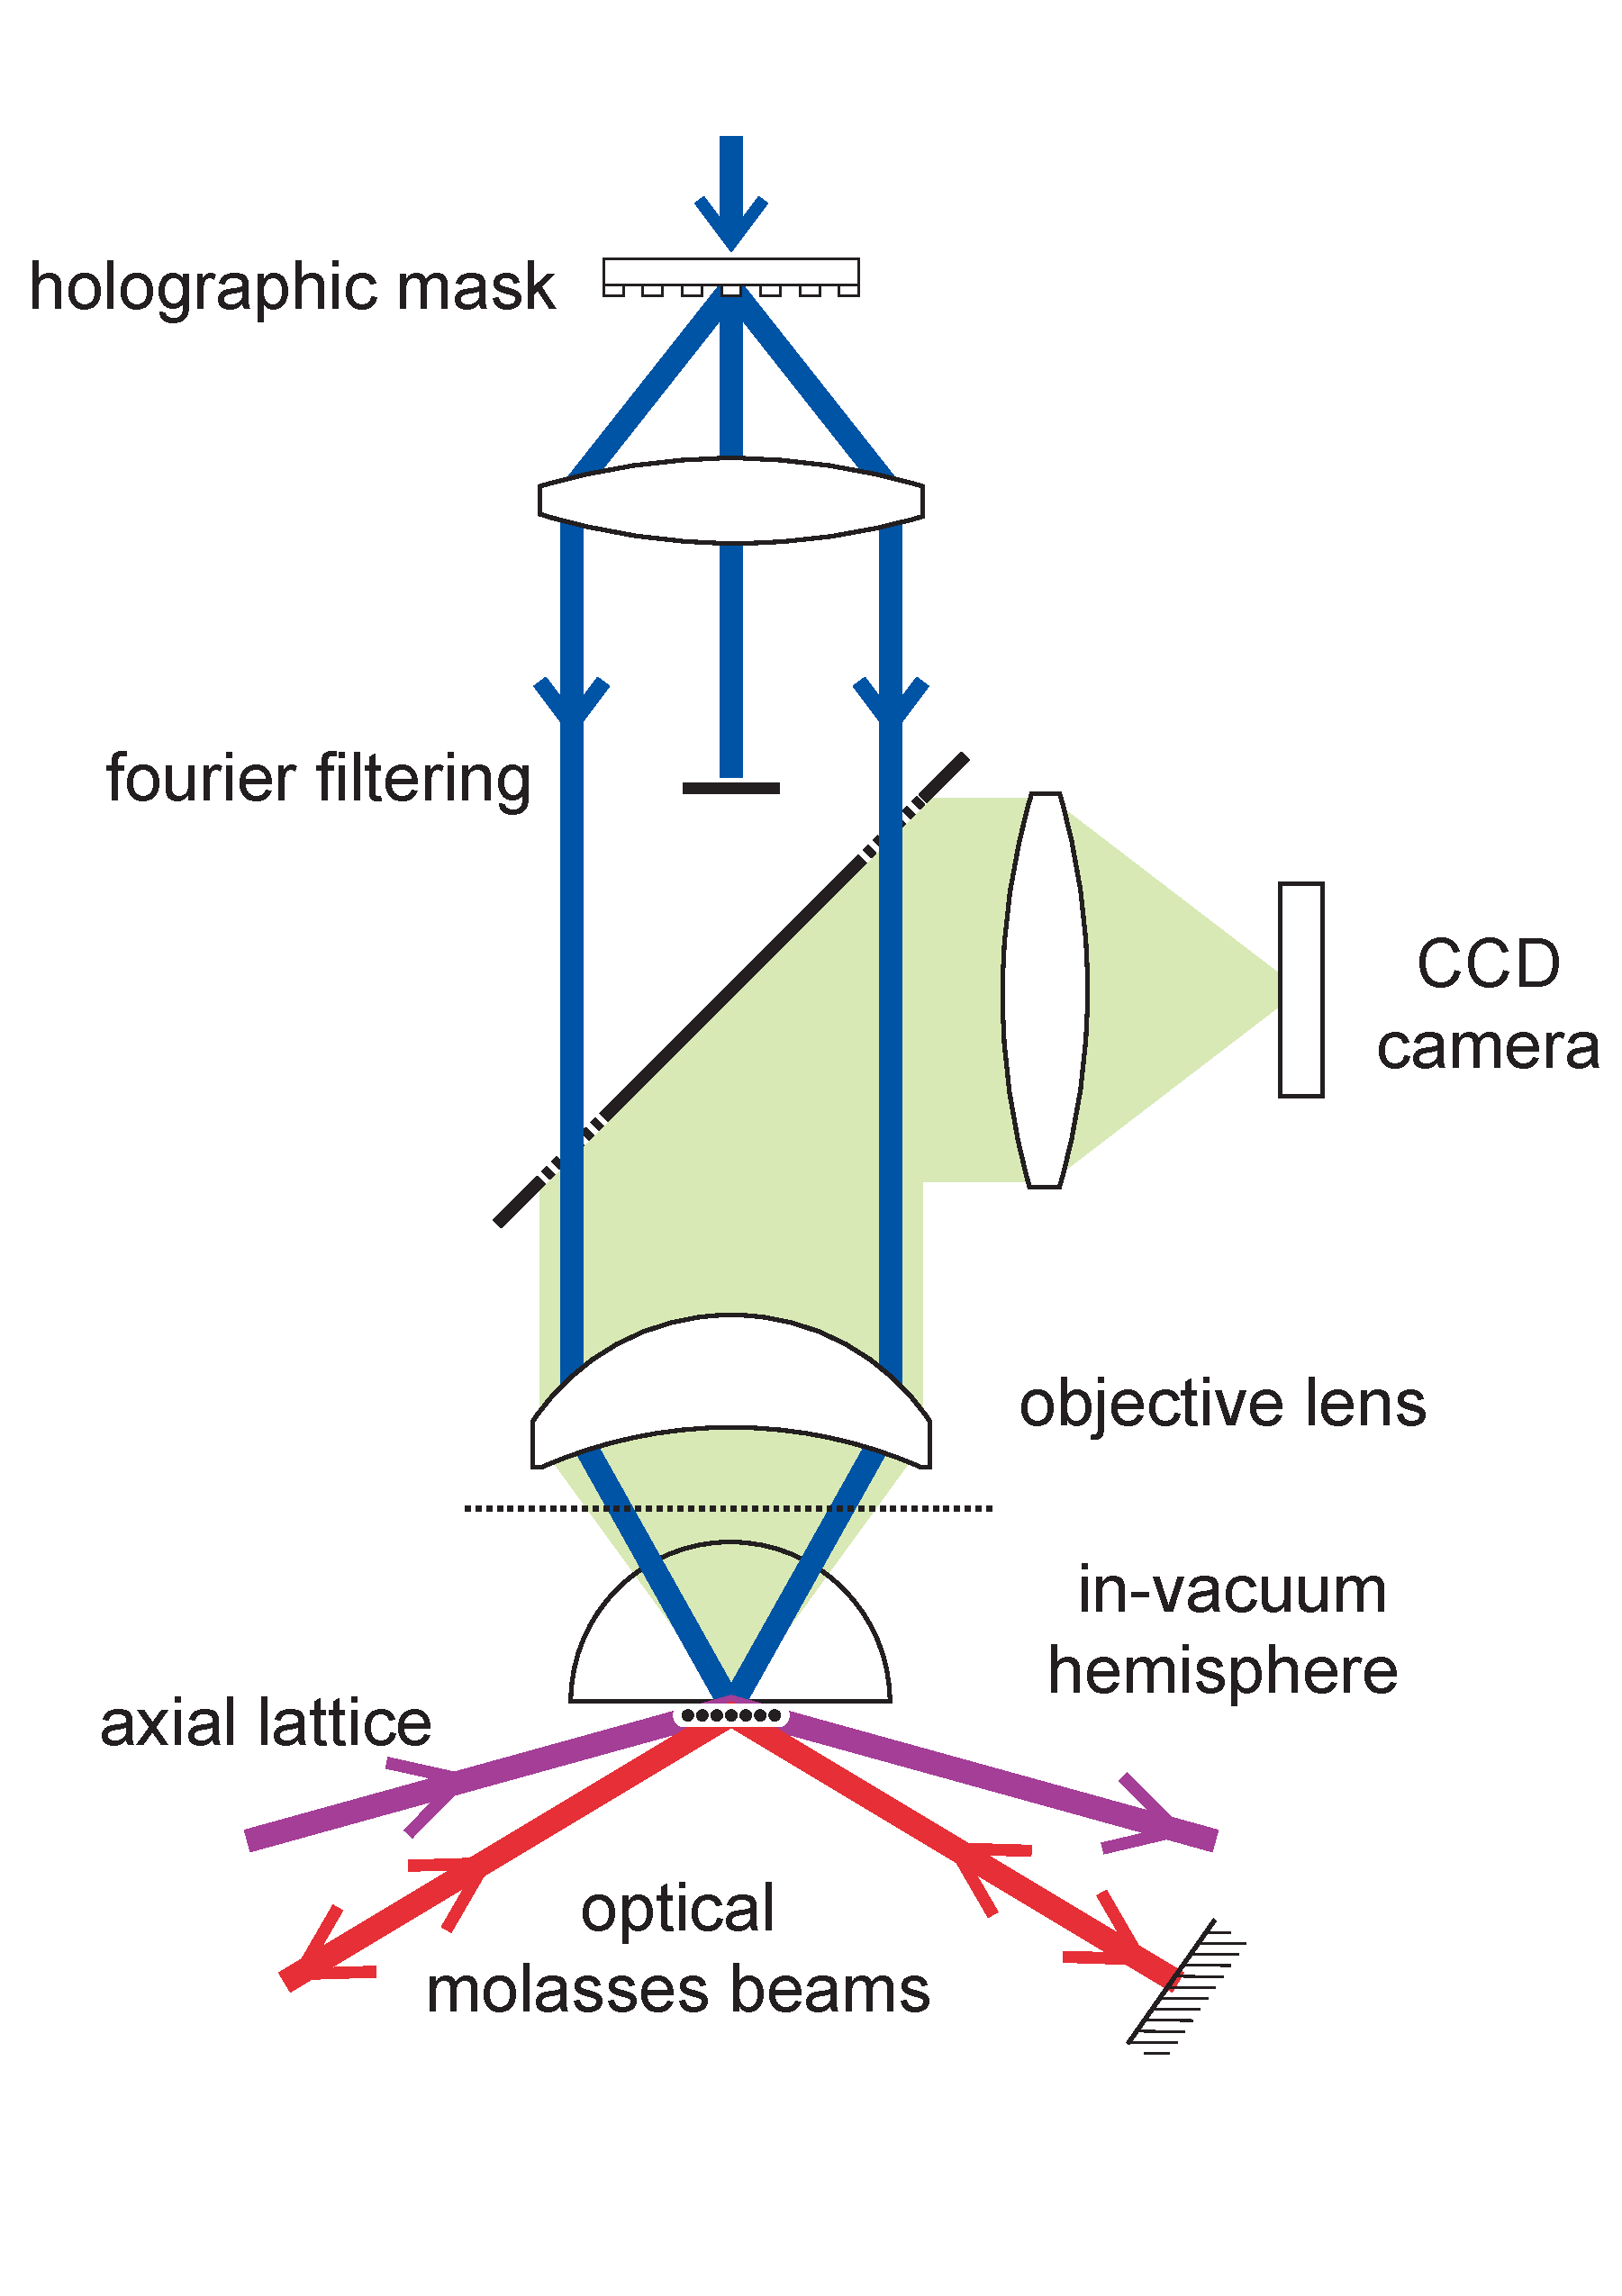
\includegraphics[width=70mm]{figures/QGM_setup.pdf}
	\caption{{\bf Schematic of the quantum gas microscope}. The two-dimensional atomic cloud of $^{87}\mathrm{Rb}$ is trapped $10\mathrm{\mu m}$ below the surface of the in-vacuum hemisphere. The vertical confinement is provided by axial lattice beams (purple) reflected at the hemisphere under a shallow angle, as are the molasses beams for fluorescence imaging (red). The square lattice (blue) is generated by holographic masks and projected through the microscope objective, which is also used to image atoms (light green path). Figure adapted from \cite{Bakr2009}.}
	\label{fig:QGM_QGM}
\end{figure*}

In the heart of the experiment we have a long working distance microscope objective with $\textrm{NA} = 0.55$ outside the vacuum glass cell. Inside the glass cell, there is a hemispherical lens made out of the material with an index of refraction $n=1.45$, mounted on top of the super polished substrate (see fiq.~\ref{fig:QGM_QGM}). The atoms a confined to the $6\mathrm{th}$ minimum of $1.5\mathrm{\mu m}$ spacing optical lattice, $10\mathrm{\mu m}$ below the super-polished substrate. Refraction on the bottom of the hemisphere leads to an effect similar to 'solid immersion', which increase the NA of the combined imaging system to $0.8$. The resulting diffraction-limited resolution at the $D2$ transition line of $^{87}\mathrm{Rb}$ ($\lambda = 780\mathrm{nm}$) is $600\mathrm{nm}$. 

Unlike the typical lattice experiments, where the lattice potential is created by retroreflecting the laser beam onto itself. We utilize the high numerical aperture of our imaging system, to create the $2D$ lattice by $4\mathrm{f}$ imaging a pair of holographic masks with additional Fourier filtering (see fiq.~\ref{fig:QGM_QGM}). The resulting potential has a lattice spacing of $\sim 680\mathrm{nm}$, which gives the recoil energy in both directions of $E_r = 2\pi \cdot 1240\mathrm{Hz}$.

This technique has one major advantage and one drawback. The advantage is that the lattice spacing in the image plane does not depend on the wavelength of the lattice light. This effect is due to the property of $4\mathrm{f}$ imaging system. As we discuss below, it allows us to increase the depth of the lattice by several orders of magnitude without increasing the light intensity on the atoms. However, the disadvantage is that the resulting potential has slow varying random offsets due to the interference of the lattice beams with the stray light. In order to decrease the amount of disorder in the system, we rely on the wavelength insensitivity of this technique in order to produce the lattice with $\sim 3\mathrm{nm}$ broad light source with the central wavelength of $\sim 760\mathrm{nm}$ in combination with additional spatial filtering in the Fourier plane. This allows us to eliminate some of the unwanted interference effects of the light, reflected from the optical surfaces along the imaging path. Further details on how to improve the quality of projected potential can be found in the thesis of Ruichao MA \cite{MaThesis}.

\section{Single-site resolved imaging}
In order to image the atoms at the end of the experiment, the depth of the $2D$ lattice is rapidly increased to $\sim 5000 E_r$, which freezes the tunnelling in the $x-y$ plane. This is done by switching the lattice light to $\sim 30\mathrm{GHz}$ blue detuned from the Rubidium $D1$ line ($\lambda = 795\mathrm{nm}$). Since the lattice light is close detuned the effects of spontaneous emission are not negligible anymore. In order to prevent the atoms form heating \cite{Gerbier2010,Pichler2010}, which would lead to their loss from the lattice, we cool the atoms using $80\mathrm{MHz}$ detuned optical molasses on the $D2$ line ($\lambda = 780\mathrm{nm}$). 

\begin{figure*}[t]
	\centering
	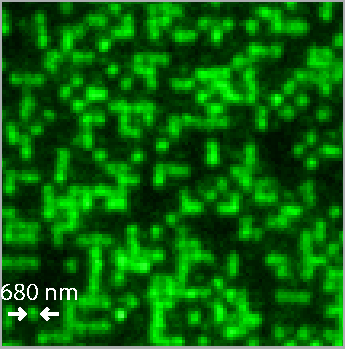
\includegraphics[scale=1]{figures/QGM_atoms.pdf}
	\caption{{\bf Single shot image of individual atoms in the optical lattice}. Green spots correspond to fluorescence collected from individual sites of the optical lattice. The underlying square geometry is visible from the picture. Due to the parity projection each site appears either bright or dark. Figure adapted from \cite{Bakr2009}.}
	\label{fig:QGM_atoms}
\end{figure*}

By collecting the photons, scattered from the molasses, on the EMCCD camera we can obtain single-site resolved images of our system (see fig.~\ref{fig:QGM_atoms}). During the typical exposure time of $500 \mathrm{ms}$ we collect $\sim 2000$ photons from individual atoms, which correspond to $\sim 10\%$ of the total number of scattered photons. 

One might notice, that the image contains two different types of site: occupied and unoccupied, although there is no restriction for multiple bosons to occupy the same site. This is due to the so-called light-assisted collisions \cite{Suominen1996,Carpentier2013}, that occur during the imaging process. When two atoms are tightly confined in space (such as in the case of the deep imaging lattice), the presence of red-detuned light makes the atoms interact via attractive dipole-dipole potential. The energy release from such a process gives them enough kinetic energy to escape the optical lattice. In our parameter regime, this process happens on the $\sim100 \mathrm{ms}$ timescales, orders of magnitude faster than the time to collect enough photons for imaging. Therefore all images that we get are so-called parity projected: each site with an odd number of atom appears bright whereas sites with even number appear dark. 

The obtained image is analyzed by fitting the amplitude of separately determined point spread function on each individual lattice site. The amplitude distribution has a clear bimodal structure \cite{Bakr2009}, therefore can be easily binarized. The fidelity of distinguishing between occupied and unoccupied sites is $>99\%$.